\documentclass{standalone}
\usepackage{tikz}
\usetikzlibrary{shapes.geometric, arrows}

\definecolor{pantone}{RGB}{63,173,168}
\definecolor{darkred}{RGB}{173,63,68}
\tikzstyle{block} = [rectangle, rounded corners, minimum width=4cm, minimum height=1.5cm,text centered, draw=black, fill=pantone, ultra thick]
\tikzstyle{arrow} = [thick,->,>=stealth]

\begin{document}

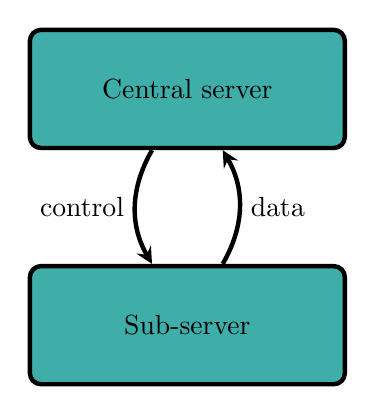
\begin{tikzpicture}[node distance=3cm]

\node (centralserver) [block] {Central server};
\node (subserver) [block, below of=centralserver] {Sub-server};

\draw [arrow, bend right, ultra thick] (centralserver) edge node[anchor=east] {control} (subserver);
\draw [arrow, bend right,ultra thick] (subserver) edge node[anchor=west] {data} (centralserver);

\end{tikzpicture}

\end{document}